\documentclass[a4paper,10pt,fleqn,twocolumn,twoside]{scrartcl}
\usepackage[utf8]{inputenc}
\usepackage[T1]{fontenc}

\usepackage{lmodern}
\usepackage[scaled=0.80]{DejaVuSans}

\usepackage{ngerman}
\usepackage{amsmath}
\usepackage{amssymb}
\usepackage{booktabs}
\usepackage{microtype}
\usepackage{color}
\definecolor{c1}{RGB}{00,40,80}
\usepackage[colorlinks=true,linkcolor=c1]{hyperref}
\usepackage{geometry}
\geometry{a4paper,left=25mm,right=15mm,top=20mm,bottom=28mm}
\setlength{\columnsep}{6mm}
\usepackage{graphicx}
\numberwithin{equation}{section}

\begin{document}
%\thispagestyle{empty}

\noindent
\textbf{\sffamily\huge Elektrotechnik}\\
\\
Februar 2016
\vspace{1em}

\noindent
Dieser Text steht unter der Lizenz\\
Creative Commons CC0.


\tableofcontents
%\newpage

\section{Kapazitäten}
\subsection{Ein Kondensator entlädt sich}

\begin{figure}[h]
\centering
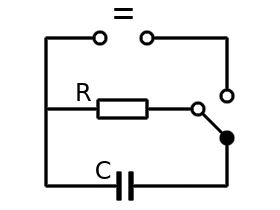
\includegraphics[width=42mm]{img/RC.png}
\caption{RC-Masche}
\label{RC}
\end{figure}

\noindent
Der Kondensator wurde vollständig geladen und hat die Spannung
$U_0$. Es fließt ein Anfangsstrom durch den Widerstand, welcher
durch $U_0=RI_0$ beschrieben wird. Nach dem Maschensatz
gilt $u_R+u_C=0$.
Die Gleichung wird auf beiden Seiten abgeleitet und man erhält
$u_R'(t)+u_C'(t)=0$. Nun verwendet man $u_R=Ri_R$ und $i_C=Cu_C'(t)$.
Bedenkt man nun, dass $i_R=-i_C$ gilt, so gelangt man zur
Differentialgleichung%
\begin{equation}
RCi_R'(t) = i_R(t).
\end{equation}
Das ist eine lineare GDG erster Ordnung mit konstanten Koeffizienten.
In der Form $y'(t)=ay$ hat sie die allgemeine Lösung
$y(t)=y(0)e^{at}$. Wir betrachten nun nur die Stromstärke am
Widerstand und setzen $i:=i_R$. Damit ergibt sich%
\begin{equation}\label{RCStrom}
i(t) = I_0\exp\Big(-\frac{t}{RC}\Big)
\end{equation}
Nun wollen wir wissen, wie viel Ladung im geladenen Kondensator
steckt. Dazu bedenkt man, dass $Q=It$ gilt, falls die Stromstärke
zeitlich konstant ist. Für eine veränderliche Stromstärke $i(t)$
kann die Ladung als der Flächeninhalt unter der Kurve $i(t)$
betrachtet werden. Für das Intervall $[0,t]$ ergibt sich also
der Flächeninhalt%
\begin{gather*}
Q([0,t]) = \int_0^t I_0 \exp\Big(-\frac{x}{RC}\Big)\,\mathrm dx\\
= I_0\Big[-RC\exp\Big(-\frac{x}{RC}\Big)\Big]_{x=0}^{x=t}\\
= RC I_0 \Big[1-\exp\Big(-\frac{t}{RC}\Big)\Big].
\end{gather*}
Für $t\rightarrow\infty$ ergibt sich dann die gesamte gespeicherte
Ladung. Es ergibt sich%
\begin{equation}
Q = \lim_{t\rightarrow\infty}Q([0,t]) = RCI_0.
\end{equation}
Die gespeicherte Ladung sollte eigentlich nicht vom Widerstand
$R$ abhängig sein. Das ist sie tatsächlich auch nicht. Verwendet
man nämlich $U_0=RI_0$, so ergibt sich $Q=CU_0$. Die gespeicherte
Ladung wird also nur durch die Anfangsspannung und die Kapazität
bedingt.

Ein Kondensator ist ein Energie speicherndes Bauteil. Wie viel
Energie kann man aus einem geladenen Kondensator herausholen?
Dazu betrachten wir den Widerstand $R$ als einen Heizwiderstand.
Wir könnten $R$ elektrisch isolieren, in ein Kalorimetergefäß
mit Wasserbad stecken und schauen wie sich die Temperatur erhöht.
In der Praxis ist das ein relativ idiotischer Versuch. Man würde
dann gerne ein Beckmann"=Thermometer anschaffen um präzise zu sein,
und es muss schnell gehen, sodass man einen schnellen Rührer
benötigt. Das kann sehr teuer werden. Die letzten Dewar-Gefäße,
die ich benutzt habe, waren viel zu dünn, da haben kaum ein
Thermometer und ein Rührer gleichzeitig Platz. Man läuft Gefahr,
mit dem Rührer das Beckmann abzurasieren. 

Für eine konstante Leistung ist $W=Pt$. Nun wenn $p(t)$ die
Momentanleistung am Widerstand ist, so ergibt sich die gespeicherte
Energie wieder als Flächeninhalt unter der Kurve $p(t)$.
Weiterhin gilt $p(t)=u(t)i(t)$. Mit $u=Ri$ bekommt man
$p(t)=Ri(t)^2 t$. Schaut man sich (\ref{RCStrom}) an, so sieht man
wegen $(e^x)^2=e^{2x}$ ein, dass bei der Integration lediglich
die Zwei beachtet werden muss. Man verwendet die Substitution
$x=2y$. Hiermit ist $\mathrm dx=2\mathrm dy$ und es ergibt sich%
\begin{gather*}
W([0,t]) = \int_0^t RI_0^2 \exp\Big(-\frac{2y}{RC}\Big)\,\mathrm dy\\
= \frac{RI_0}{2}\int_0^{2t} I_0 \exp\Big(-\frac{x}{RC}\Big)\,\mathrm dx
= \frac{RI_0}{2}Q([0,2t]).
\end{gather*}
Lässt man $t\rightarrow\infty$ gehen, so ergibt sich%
\begin{equation}
W = \frac{1}{2}RI_0Q = \frac{1}{2}QU_0 = \frac{1}{2}CU_0^2.
\end{equation}
Ein Kondensator ist im Gegensatz zu einem Akkumulator ein Bauteil,
welches Energie sehr schnell aufnehmen und abgeben kann. Das macht
sich in der Praxis auch maßgeblich bemerkbar. So kann man z.B. schon
von mittelgroßen ausreichend geladenen Elkos eine gewischt bekommen.
Beliebt ist der Versuch einen Aluminiumring auf einem
Permanentmagneten mit der lenzschen Regel in die Luft werfen zu
lassen. Hierfür braucht man sehr schnell einen großen Strom, wofür
man am besten einen Kondensator verwendet.

Wenn Kondensatoren eine ausreichende Kapazität und
Durchschlagsfestigkeit haben, sind diese im geladenen Zustand
sehr gefährlich. Man muss Apparaturen vollständig abisolieren
und nach einem Versuch alle Kondensatoren entladen lassen.
Hier gilt wie immer Murphys Gesetz.

Für selbstgebaute Teslaspulen haben Leute für den Primärkondensator
ein Array aus kleistschen Flaschen verwendet, die aus Trinkflaschen
selbst baut wurden. Schon eine einzige kleistsche Flasche ist
gefährlich, wenn sie ausreichend lange mit Hochspannung geladen wird.


\subsection[Ein Kondensator im Wechselstromkreis]%
{Ein Kondensator im Wechselstromkreis}

Ein Kondensator wird an eine Stromquelle angeschlossen.
Das Amperemeter wird zum Kondensator in Reihe geschaltet.
Das Voltmeter in Parallelschaltung.

Legt man an einem Kondensator eine Gleichspannung an, so wird er eine
Weile aufgeladen. Während er sich auflädt, fließt ein Ladestrom.
Nachdem er sich aufgeladen hat natürlich nicht mehr. Legt man den
Kondensator aber an eine Wechselspannung mit genügender Frequenz,
dann fließt der Ladestrom immer. Wie ist dieses Verhalten zu
erklären?

Ok es ist schon ziemlich offensichtlich. Da die Spannung ständig
umgepolt wird, lädt und entlädt sich der Kondensator auch ständig.
Man misst dann bei genügender Frequenz den Effektivwert
der Stromstärke. Wir versuchen nun eine exakte Gleichung für die
Stromstärke aufzustellen. Damit können wir eine Gleichung
für den Effektivwert gewinnen.

Die Stromstärke gibt an, wie viel Ladung in einer bestimmten Zeit
bewegt wird. Lassen wir die Differenz der Zeit gegen null gehen,
so gilt $i=Q'(t)$. Das $i$ für die Stromstärke wird klein
geschrieben, um anzudeuten, dass sie variiert. Die Ladung ist nach
der Definitionsgleichung für die Kapazität gegeben durch
$Q(t)=CU(t)$ und wird eingesetzt, man erhält%
\begin{equation}
i(t) = \frac{\mathrm d}{\mathrm dt}(CU(t)) = CU'(t).
\end{equation}
Nun die Gleichung für eine Sinusspannung einsetzen, es ergibt sich%
\begin{equation}
i(t) = C\frac{\mathrm d}{\mathrm dt}
(\hat u\,\sin(\omega t)).
\end{equation}
Mit der Kettenregel erhält man
\begin{equation}
i(t) = C\hat u \omega\,\cos(\omega t).
\end{equation}
Nun handelt es sich bei den Vorfaktoren um die
Amplitude der Stromstärke, d.h. es ist
$\hat i=C\hat u\omega$. Die Gleichung bekommt damit
die Form%
\begin{equation}
i(t) = \hat i\,\cos(\omega t).
\end{equation}
Hiermit ergibt sich schließlich
\begin{equation}
I_{\mathrm{eff}} = CU_{\mathrm{eff}}\omega.
\end{equation}
Wie erwartet, hängt der Effektivwert von der Kreisfrequenz
ab. Besonders interessant ist weiterhin, dass auch die gemessene
Stromstärke sinusförmig ist.

\section{Dioden}
\subsection{Diode an einer Wechselspannung}
\begin{figure}[h]
\centering
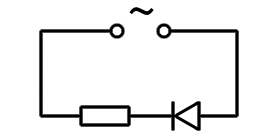
\includegraphics[width=42mm]{img/DiodeR.png}
\caption{Diode und Widerstand}
\label{DiodeR}
\end{figure}

\noindent
Betrachten wir eine Diode an einer Wechselspannung. Eine ideale
Diode wird durch die Schockley"=Gleichung%
\begin{equation}
i=I_S(e^{\lambda u}-1)
\end{equation}
beschrieben. Setzt man für $u$ die Sinusspannung
$\hat u\sin(\omega t)$ ein, so sieht man dass durch die
Schockley"=Gleichung eine Gleichrichtung der Stromstärke
beschrieben wird. Dazu plottet man exemplarisch
$u(x):=4\sin(x)$ und nimmt $\lambda:=1$ sowie $I_S:=1/10$.
Hiermit ergibt sich%
\begin{equation}
i(x)=\frac{1}{10}[e^{4\sin(x)}-1].
\end{equation}
Zur Diode schalten wir nun einen Widerstand in Reihe.
Welche Stromstärke erhält man? Welche Spannung misst man am
Widerstand? Nach dem Maschensatz gilt zunächst%
\begin{equation}
u_q+u_R+u=0,
\end{equation}
wobei mit $u$ die Spannung an der Diode gemeint ist.
Verwendet man noch $u_R=Ri$, so ergibt sich
für die Stromstärke die Gleichung%
\begin{equation}\label{eq:impliziti}
i=I_S[\exp(-\lambda(u_q+Ri))-1].
\end{equation}
Durch diese Gleichung ist $i$ implizit dargestellt. Man kann
die Kurve $i(t)$ mit einem Plotter für implizite Funktionen
plotten und lösen, denn wir haben hier eine implizite
Funktion $F(i,t)=0$. Für einen
beispielhaften Plot nimmt man alle Parameter wie bisher, das
sind $u_q:=4\sin x$, $I_S:=1/10$ und
$\lambda:=1$. Man kann $\omega:=1$ setzen, sodass $x=t$ gilt.
Für den Widerstand nimmt man am besten einfach $R:=1$.

Für die Spannung am Widerstand ergibt sich%
\begin{equation}\label{eq:DiodeuR}
u_R = -u_q -\frac{1}{\lambda}\ln\Big[\frac{u_R/R+I_S}{I_S}\Big].
\end{equation}
Hierdurch wird $u_R$ implizit beschrieben.

Wir wollen die Gleichung für $i$ lösen. Dazu approximiert man für
$I_S\ll 1$ die Schockley-Gleichung durch $i\approx I_S e^{\lambda u}$.
Gleichung (\ref{eq:impliziti}) wird nun zu%
\begin{equation}\label{eq:iapprox}
i=I_Se^{-\lambda u_q}e^{-\lambda Ri} = Ke^{-\lambda Ri}.
\end{equation}
Diese Gleichung lässt sich mit der Lambert-W-Funktion lösen.
Die Lambert-W-Funktion $x=W(y)$ ist die Umkehrfunktion von
$y=xe^x$. Aus (\ref{eq:iapprox}) ergibt sich durch Umformung%
\begin{equation}
\lambda RK = \lambda Rie^{\lambda Ri}.
\end{equation}
Das gerade die Gleichung, welche man durch die Lambert-W-Funktion
lösen kann. Man erhält%
\begin{equation}
i = -\frac{1}{\lambda R}W(\lambda RK).
\end{equation}
Für das konkrete Beispiel hat man
\begin{gather*}
K:=I_S e^{-\lambda u_q} = \frac{1}{10}e^{-4\sin x},\\
\lambda R = 1.
\end{gather*}
Damit erhält man die Lösung
\begin{equation}
i(x) = W[\exp(-4\sin x)\big].
\end{equation}
Bei Octave und Matlab heißt der obere Ast der Funktion
\texttt{lambertw}. Bei Octave muss man noch das Paket
\texttt{specfun} nachinstallieren. Man kann $W(x)$ aber auch
selbst approximieren. Dazu nimmt man zunächst die Approximation%
\begin{equation}\label{Wapprox}
W(x)\approx \ln\sqrt{2x+1}.
\end{equation}
Aus der Gleichung $x=W(x)e^{W(x)}$ bekommt man%
\begin{equation}
W(x) = \ln\Big(\frac{x}{W(x)}\Big),
\end{equation}
was als Fixpunktiteration für $W(x)$ benutzt werden kann.
Nach einer Iteration gelangt man zu%
\begin{equation}
W(x)\approx \ln\bigg(\frac{x}{\ln\sqrt{2x+1}}\bigg).
\end{equation}
Mit dem Newtonverfahren bekommt man die Fixpunktiteration%
\begin{equation}
\varphi(W) = W-\frac{W-xe^{-W}}{W+1}.
\end{equation}
Hiermit bekommt man nach zwei bis vier Iterationen eine sehr gute
Näherung aus der Anfangsnäherung (\ref{Wapprox}). Mit dieser
Iteration wird bis auf die nähere Umgebung der Verzweigungsstelle
$x=-1/e$ und des Unendlichen $x\rightarrow\infty$ der gesamte
obere Ast von $W(x)$ beliebig gut approximiert.

Die Näherung (\ref{Wapprox}) reicht für die Betrachtung des
qualititativen Verhaltens von (\ref{eq:impliziti}) bereits aus.

Die Gleichung (\ref{eq:impliziti}) kann mit der Lambert-W-Funktion
aber auch exakt gelöst werden. Dazu macht man die Substitution
$j:=i-I_S$. Definiert man die Abkürzung%
\begin{equation}
K:=I_s\exp(-\lambda u_q-\lambda RI_s),
\end{equation}
so gelangt man zu $j=Ke^{-\lambda Rj}$. Diese Gleichung lässt sich
wieder in die Form $\lambda RK=\lambda Rje^{\lambda Rj}$
bringen. Es ergibt sich $\lambda Rj=W(\lambda RK)$ und
nach Resubstitution%
\begin{equation}
i = \frac{1}{\lambda R}W(\lambda RK)+I_s.
\end{equation}
Die Gleichung (\ref{eq:DiodeuR}) bringt man erst einmal in die
Form%
\begin{equation}
(u_R+RI_S)\exp(\lambda u_R+\lambda u_q) = RI_S.
\end{equation}
Jetzt verwendet man die Substitution
$v:=u_R+RI_S$. Damit gelangt man zur Gleichung%
\begin{equation}
\lambda ve^{\lambda v}=K'
\end{equation}
mit
\begin{equation}
K':=\lambda RI_S\exp(\lambda RI_S-\lambda u_q).
\end{equation}
Mit $\lambda v=W(K')$ ergibt sich nach Resubstitution%
\begin{equation}
u_R = \frac{1}{\lambda} W(K')-RI_S.
\end{equation}

\subsection{Vergleich mit einer realen Diode}
An dieser Stelle soll überprüft werden, ob sich eine
reale Diode einigermaßen vernünftig mit der Schockly-Gleichung
beschreiben lässt. Ich habe dazu noch einige Messwerte für
die Diode \texttt{SY223 CK}. Das ist eine Siliziumdiode, die noch
in der DDR produziert wurde. Die Germaniumdioden werden als
\texttt{GY100} bis \texttt{GY125} bezeichnet. Die Messwerte wurden
leider unter sehr widrigen Umständen aufgenommen. Ich habe so ein
Multimeter für 5\,EUR benutzt, welches ich mir geliehen hatte.
Ich muss auf die Angabe von Fehlergrenzen daher verzichten.

Die Messwerte sind folgende:

{\normalfont\ttfamily
\begin{tabular}{r|l}
$u/\mathrm{mV}$ & $i/\mathrm{mA}$\\
300 & 0.010\\
350 & 0.025\\
400 & 0.055\\
450 & 0.160\\
500 & 0.410
\end{tabular}
}

\noindent
Der Graph scheint einen exponentiellen Zusammenhang zu
beschreiben. Da sowieso nicht erkennbar ist, dass $i(u)$ irgendwo
negativ wird, benutzt man das vereinfachte Modell
$i=I_Se^{\lambda u}$. Logarithmiert man diese Gleichung auf
beiden Seiten, so erhält man%
\begin{equation}
\ln i = \ln I_S + \lambda u.
\end{equation}
Man sieht, $\ln i$ ist eine affine Funktion von $u$. Man kann lineare
Regression benutzen. Man berechnet dazu%
\begin{equation}
y(x) = \overline y+\frac{s_{xy}}{s_x}(x-\overline x).
\end{equation}
Die Berechnung ergibt:
\begin{gather*}
\overline x = 400\,\mathrm{mV}\\
\overline y = -2.78+\ln(\mathrm{mA})\\
s_{xy}/s_x = 0.0186/(\mathrm{mV})
\end{gather*}
Damit ergibt sich $\lambda = 0.0186/(\mathrm{mV})$ und\\
$I_S=3.64\times 10^{-5}\,\mathrm{mA}$.
Der empirische Korrelationskoeffizient ist%
\begin{equation}
r_{xy} = \frac{s_{xy}}{\sqrt{s_x s_y}} = 0.9990
\end{equation}
Geht man nun davon aus, dass die Diode nicht besonders hochwertig
gefertigt ist, so sollte man für den Emissionskoeffizienten $n$
eher $n=2$ wählen. Damit ergibt sich eine Temperaturspannung von%
\begin{equation}
U_T = \frac{1}{2\lambda} = 26.9\,\mathrm{mV}.
\end{equation}
Für die größte Aufheizung der Diode bei den Messwerten ergibt
sich eine Leistung von $0.2\,\mathrm{mW}$. Das ist wohl
vernachlässigbar und man kann somit die Umgebungstemperatur
abschätzen. Es ergibt sich%
\begin{equation}
T = \frac{q_e U_T}{k_B} = 312\,\mathrm{K}.
\end{equation}
Man bekommt $\theta = 39\,\mathrm{{}^\circ C}$, was wohl etwas
zu warm ist. Geht man umgekehrt von $25\,\mathrm{mV}$
Temperaturspannung bei Zimmertemperatur aus, so ergibt
sich $n=2.15$ anstelle von $n=2$. Das ist ersichtlich, weil
die Exponentialfunktion Fehler erheblich vergrößert.

Die Daten in Tabelle \ref{table:SY} findet man auf dem
Originaldatenblatt »\texttt{SY220}{\ldots}\texttt{SY230},
Silizium"=Gleichrichterdioden für Ströme bis 1\,A«.

\begin{table}[t]
\begin{tabular}{rl}
\toprule
$\hat U_{RN} = 300\,\mathrm{V}$ & Nennsperrspannung\\
$U_R = 300\,\mathrm{V}$ & Sperrgleichspannung\\
$\hat U_{RP} = 390\,\mathrm{V}$ & Periodische Spitzenspannung\\
$\hat U_{RS} = 450\,\mathrm{V}$ & Stoßspannung\\
\midrule
$\hat U_F \le 1.2\,\mathrm{V}$ & Durchlaßspannung\\
$U_S = 0.8\,\mathrm{V}$ & Schleusenspannung\\
$\overline I_{FN} = 0.7\,\mathrm{A}$
  & Nenndurchlaßstrom (R-Last)\\
$\overline I_{FN} = 0.6\,\mathrm{A}$
  & Nenndurchlaßstrom (C-Last)\\
\midrule
$I_{FM} = 2\,\mathrm{A}$ & Dauergrenzstrom\\
$\overline I_{FP}=8\,\mathrm{A}$
  & Period. Spitzendurchlaßstrom\\
$\overline I_{FS}=40(50)\,\mathrm{A}$
  & Stoßstrom\\
$\ddot U = 8(12.5)\mathrm{A^2 s}$
  & Grenzstromintegral\\
\midrule
$I_F \le 0.15\,\mathrm{mA}$ & Sperrstrom\\
$r_F \approx 70\,\mathrm{m\Omega}$
  & Diff. Durchlaßwiderstand\\
$C_0 \approx 50\,\mathrm{pF}$
  & Nullpunktkapazität\\
$R_{\mathrm{th}}{\le}100\,\mathrm{grd/W}$
  & Gesamtwärmdewiderstand\\
\midrule
$-40{\ldots}{+}150\,\mathrm{{}^\circ C}$
  & Betriebstemperaturbereich\\
$m=3\,\mathrm{g}$ & Masse\\
\bottomrule
\end{tabular}
\caption{SY220{\ldots}SY230, Silizium"=Gleichrichterdioden
für Ströme bis 1\,A}
\label{table:SY}
\end{table}
Es folgen noch Referenzen auf TGL-Normen und
wei Diagramme für die Silizium"=Gleichrichterdiode \texttt{SY201}.
Das erste, »Durchlaßverlustleistung in Abhängigkeit des
Durchlaßstrommittelwertes, Parameter: Duchlaßwinkel
$\varrho$«, zeigt  $P_F(J_F)$ mit $P_F$ in~W und $J_F$ in~A.

Das zweite, »Zulässige Verlustleistung
in Abhängigkeit von der Umgebungstemperatur, Parameter:
Sperrschichttemperatur $\theta_j$«, zeigt $P(\theta)$
mit $P$ in~W und $\theta$ in ${}^\circ\mathrm{C}$.

Die Schleusenspannung $U_S$ erhält man,
wenn man bei genügend hohem Anstieg von $i(u)$ eine Tangente
zieht. An der Kennlinie sieht man, dass man den Differenzenquotient
der letzten beiden Messwerte bilden kann. Es ergibt sich etwa
$425\,\mathrm{mV}$. Im Datenblatt ist aber $800\,\mathrm{mV}$
angegeben. Der Wert ist jedoch auch in erheblichem
Maß davon Abhängig, welche $y$-Skalierung man verwendet.
Das macht diese Methode praktisch unbrauchbar.

Für diese Methode soll kurz noch eine Formel entwickelt werden,
mit der man die Schleusenspannung berechnen kann, ohne
auf eine Kennlinie zu schauen. Die Krümmung des Graphen kann für den
Bereich durch%
\begin{equation}
K = \frac{f''(x)}{f'(x)^3}
= \frac{I_S\lambda^2 e^{\lambda x}}{I_S^3\lambda^3 e^{3\lambda x}}
= \frac{1}{I_S^2\lambda e^{2\lambda x}}
\end{equation}
mit $x=u$ approximiert werden. Die Krümmung sollte ausreichend
klein sein, so dass man ein $u_0$ erhält.
Dann lässt sich eine Tangente anlegen, welche
durch die Gleichung%
\begin{equation}
T(u) = I_S e^{\lambda u_0}+I_S \lambda e^{\lambda u_0}(u-u_0)
\end{equation}
beschrieben wird. Die Tangentenfunktion hat die Nullstelle%
\begin{equation}
U_S = u_0-\frac{1}{\lambda} = \frac{1}{2\lambda}
\ln\bigg[\frac{1}{KI_S^2\lambda}\bigg]-\frac{1}{\lambda}.
\end{equation}
Misst man $u$ in mV und $i$ in mA, so kann man eine passende
Krümmung $K$ wählen. Diese ergibt sich mit%
\begin{equation}
\frac{1}{K} = I_S^2\lambda\exp(2\lambda U_S+2).
\end{equation}
Für $U_S=425\,\mathrm{mV}$ bekommt man hier $K=3500$.

Verwendet man für $U_S$ stattdessen den Wert, welcher sich
bei $i=1\,\mathrm{mA}$ ergibt, so erhält man%
\begin{equation}
U_S = \frac{1}{\lambda}\ln(i/I_S) = 560\,\mathrm{mV},
\end{equation}
was immer noch viel geringer als auf dem Datenblatt ist.

\subsection{Lineares Modell für die Diode}
Die Diode kann man im Arbeitsbereich linearisieren.
Hier wählt man für die Knickstelle eine Spannung $u_0$,
die mit der Schleusenspannung übereinstimmt oder kurz davor
liegt. Vor dieser Knickstelle setzt man $i(u)=0$. Danach
wählt man einen bestimmten differentiellen Leitwert $g$
als Anstieg für die Gerade. Das lineare Modell lautet
damit%
\begin{equation}
i(u) = [u>u_0]g(u-u_0),
\end{equation}
wobei mit $[A]$ die Iverson"=Klammer gemeint ist.

\end{document}


